\documentclass[10pt,a4paper]{article}

\usepackage{graphicx}                                                   % load and handle pictures
\graphicspath{{./figs/}}                                                % look for images here

\usepackage{url}                                                        % nicely formatted URL's
\usepackage[textwidth=\marginparwidth + 2cm]{todonotes}                 % insert to–do and missing figure items in the document
  \newcommand{\addref}{\todo[color=red!40,size=\tiny]{Add reference}}   % new command for box about missing references
  \newcommand{\rewrite}[2][]{\todo[inline,color=green!40,#1]{#2}}       % new command for boxes of text that needs to be rewritten
  \newcommand{\think}[2][]{\todo[caption={#2}, size=\small, #1]{\renewcommand{\baselinestretch}{0.5}\selectfont#2\par}}

\newcommand{\HOneArgLysRatio}{???}
\newcommand{\OthersArgLysRatio}{???}

\newcommand{\CodingGenesInHistOne}{50}
\newcommand{\PseudoGenesInHistOne}{9}
\newcommand{\TotalGenesInHistOne}{59}

\newcommand{\CodingGenesInHistTwo}{11}
\newcommand{\PseudoGenesInHistTwo}{7}
\newcommand{\TotalGenesInHistTwo}{XXXXX}

\newcommand{\CodingGenesInHistThree}{3}
\newcommand{\PseudoGenesInHistThree}{XXXX}
\newcommand{\TotalGenesInHistThree}{XXXXX}

\newcommand{\CodingGenesInHistFour}{1}
\newcommand{\PseudoGenesInHistFour}{XXXX}
\newcommand{\TotalGenesInHistFour}{XXXXX}

\newcommand{\HistOneSpan}{2.3\,Mbp}
\newcommand{\HistTwoSpan}{105\,kbp}
\newcommand{\HistThreeSpan}{XXXXbp}
\newcommand{\HistFourSpan}{XXXXbp}


\begin{document}
  \section{Introduction}
  \label{sec:intro}
    %% Complementary introduction on the chromatin organization and how it's dynamic
    %% Explain that despite the fact that there's 4 core histones, there's actually several isoforms of each
    %% Say that no one bothers to explain which one they are using
    %% Comment that maybe the lack of information is because they are so similiar which makes difficult most of the analysis
    %% We are going to annotate all canonical histone genes on (at least GenBank and Ensembl)

    %% short 2-3 lines on chromatin organization and dynamics}
    Histones are among the most abundant proteins in eukaryotic cells and contribute up to half
    the mass of chromatin. They define the structure and accessibility of the nucleosome as the
    fundamental unit of genome organisation. In addition, the reactive sidechains of histones
    are post-translationally modified as a nexus for signalling and potentially for heritable
    epigenetics.

    Histones have been studied for many decades as abundant proteins which were readily isolated
    due to their highly basic chemical character. Successive improvements in fractionation revealed
    5 main types under a nomenclature as histone H1, H2A, H2B, H3 and H4\cite{Histonenomenc}. An additional histone H5
    related to H1 is found in nucleus-containing avian erythrocytes and has been of research interest
    due to its elevated binding stability. Since the ratio of arginine/lysine is \HOneArgLysRatio\ for H1 and H5 these
    became known as ``lysine-rich'', whereas the remaining 4 histones with ratios \OthersArgLysRatio\ are``arginine-rich''.
    The demonstration of the nucleosome as the fundamental repeating unit of chromatin revealed that H2A,
    H2B, H3 and H4 associated as an octamer of two copies each within the nucleosome core particle,
    so they are referred to as ``core histones''. H1 and H5 associate with the linker DNA between
    nucleosome core particles, and are referred to as ``linker histones''.

    %% note on calling 'histones' to 'core histones' should be at the end of introduction and after introducing the difference
    Since we write here only about the core histones, for sake of brevity we will refer to them as simply ``histones''.

  \section{Canonical isoforms vs variants\think{maybe call this section 'histone variation'? Or 'histone variants?' ?}} 
    %% Characteristics of a variant are the fact they seem to have special functions. Emphasis that some canonical may have special functions whicyh no one bothered to check
    %% variants with extra special nomenclature are outside the histone clusters and have poly-A tails (sometimes)
    %% Complain about the lack of information on the different isoforms
    %% Complain that there's small reason to call some the .1 variant, and the others .2
    \rewrite{
      Rules and exceptions to definition of canonical and variants. Also point that the word canonical suggest antecedence which is not necessarily true (ref to our paper and Henikoff's)
    }

    Extracting histones from cells and separating them by polyacrylamide gel electrophoresis (PAGE) using
    the strongly anionic detergent sodium dodecyl sulphate (SDS) and neutral buffers gives single bands
    for each histone type. However, PAGE with acetic acid in gels containing the non-ionic detergent
    Triton X--100 and uncharged urea as denaturants (TAU or AUT) allows the separation of histones
    into multiple species due to both post-translational modifications and variations in sequence
    within types. Historically, the major species in TAU separations due to polypeptide differences
    were identified by numerical suffixes as H2A.1 and H2A.2; H2B.1 and H2B.2; and H3.1, H3.2 and H3.3\cite{Non-allelicva}.

    There are two recognised classes of histone sequence variation, ``variants'' and ``canonical'', which are distinguished
    by their regulation in humans and other metazoans (Table~\ref{tab:typical-histone-differences}).

    \begin{table}
      \centering
      \begin{tabular}{l | l | l | l | l }
        \null     & Expression              & Sequence identity & Function    & 3' UTR \\
        \hline
        Canonical & Replication Dependent   & High              & Structural  & Stem--loop  \\
        Variants  & Replication Independent & Low               & Specialized & poly-A tail \\
      \end{tabular}
      \caption{Typical vision of differences between canonical and variant histones.}
      \label{tab:typical-histone-differences}
    \end{table}

    ``Variants'' play functionally distinctive roles, have lower net abundance, and typically show less
    identity in alignments. Most are significantly expressed outside S~phase of the cell cycle and are
    referred to as ``replication independent''~(RI). They typically have unique promoter elements and their
    transcripts carry 3' polyadenylated tails.

    In contrast, ``canonical'' histones contribute to the primary function and majority of nucleosome
    structures, and their ``isoforms'' exhibit high identity in alignments. Because they are primarily
    expressed to package the duplicated genome during S~phase, and show a 35~fold increase on expression
    during this phase \cite{harris-1991}, they are referred to as ``replication dependent''~(RD) or ``replacement''
    histones. They appear to share a common promoter structure (Fig.~\ref{fig:promoter-alignment}) and
    a unique stem-loop structure in the 3' untranslated region that is the
    basis for their turnover. In general, metazoan canonical histones
    are not thought to be polyadenylated, although \textit{S.\ cerevisiae} histone transcript stability
    appears to be regulated by polyadenylation instead of RNA structures. Despite the small differences between these canonical histone isoforms,
    canonical histones are sometimes known as ``wild type'' sequences and are usually considered together
    as a single histone.

    The widespread awareness of high conservation in histone protein sequences means that the true extent
    of protein and gene sequence variation in canonical histones is often under-appreciated. Albig and 


    The genes encoding canonical histone isoforms are typically found in clusters in most eukaryotic genomes,
    possibly for regulatory and expression functions and to facilitate sequence conservation. The gene clusters
    are observed to aggregate within the nucleoplasm with processing factors as Histone Locus Bodies
    (HLBs) similar but distinct from Cajal Bodies. Human histone genes are grouped in 4 nominal clusters
    (Table~\ref{tab:histone}). The major HIST1 histone gene cluster on chromosome 6 and the secondary
    HIST2 contain contiguous high density arrays of histone genes, whereas the minor HIST3 and HIST4
    loci on chromosomes 1 and 12 have a handful of histone genes interspersed with non-histone coding genes.


    %% there's several isoforms for histones and no one bothers about them
    Fitting to their important task, histone genes and proteins show some unusual characteristics.
    One of the most blatant of them but still mostly ignored, is the existence of several unique protein
    sequences \think{should explain better that we're not talking about SNP?} that despite having
    officially different names, are grouped together and rarely identified. These histone
    \emph{isoforms} are different from the so-called histone \emph{variants} whose distinction
    is based on their 3' UTR processing and genome positioning.

    Marzluff et al (2002) is the existing reference for histone nomenclature. However, it contains
    some oversights, most likeley due to the ``draft'' status of the genome it was based on. \todo{in
    the end must recheck this list of errors} One gene
    had not been identified, some proteins have different sequences, gene names had been swapped,
    and others have been found to be pseudo-genes. Similarly, the annotation of RefSeq and SwissProt
    is not yet complete and contains some omissions for the untranslated regions.

    %% we catalogued and fixed the annotations of all replication-dependent on Entrez and Ensembl
    Since we were in a position of need of such information \think{mention that it's human only.
    After marzullf reference?} we extracted the update sequences
    from GenBank \think{and Emsembl} and finished their annotation. Having finished cataloguing
    all of them, and submitting the completed annotations, we hope to have created a useful
    reference for other researchers while raising awareness of the multitude of histone isoforms.

  \section{Overview of histone genes}
  \label{sec:overview}
    The human histones can be separated in two main groups: canonical or replication-dependent, and
    variants or replication-independent.


    Variants are the most likely with a standard gene, are considered independent from each other,
    spread around the genome and its expression is mostly independent of cell cycle \think{explain
    why mostly? Do it next paragraph when complaining the naming}. When people say H2AX that's
    a variant. Note, H2A.2 and H3.2 are not considered variants.

    Both this separation and their naming is very misleading\think{say that the fact that no one cares is proof?}
    for several reasons.
    \begin{itemize}
      \item The word canonical suggests precedence which is not necessarily true. It has been
            suggested that at least in the case of H2A, the `canonical' gene may have evolved
            from one of the `variant' genes\addref.
      \item Not all `variant' are replication-independent. H2AX gene for example expression
            increases during S--phase together with other `canonical' histones and does show
            a transcript with stem-loop.
      \item The `variant' vs `canonical' separation suggests that there's no variance inside
            the `canonical' which is false. There's several unique protein sequences for each
            `canonical' protein. And even the sometime named H2A.2 and H3.2 variants are actually
            `canonical' histone proteins.
    \end{itemize}

%    \rewrite{seems its missing here some definition of isoforms and replication-dependent or independent
%    and variants and replication-independent. But to explai that we need to explain clusters. And the line
%    cluster -> gene -> transcript -> protein will be broken}

  \section{Histone gene nomenclature}
  \label{sec:nomenclature}
    %%The histone gene names have a specific nomeclature, different for canonical and variant histones.
    Histone genes have a specific nomenclature that reflects their organization on the genome \think{possible
    confusion with specific histone distribution on chromatin?}. Albeit a bit long and confusing at first sight,
    once undersood they're logical and easy to remember\think{not really for the variants. But will we even
    talk deeply about the variant genes?}.

    A typical replication histone gene has a name such as HIST1H3B. This name can be split in 3 parts, HIST1, H3 and B.
    The first states the histone cluster it's located, the second the type of histone and the last, its position on
    the cluster taking in account mouse homologous. Some letters may be missing, e.g. HIST1H2AF, since it exists in the
    mouse genome (this is to make it easier to cross data between the two animal models).

    The names for the variants tend to be more random. With the exception of CENP--A (H3 variant named CENtromeric Protein A)
    all are named similarly to H2AFX where F stands for Family and the letters after have some historical or functional meaning.
    For example, H2AFZ was the last (hence Z) blot on a gel.

    \begin{figure}
      \centering
      
\includegraphics[width=\textwidth]{nomenclature-schematic.pdf}
      \caption{Nomenclature}
      \label{fig:nomenclature}
    \end{figure}

  \section{Histone clusters}
  \label{sec:cluster}
    %% Talk about the histone clusters and the distribution of each histone
    The human histone genes are organized in 4 clusters (HIST1, HIST2, HIST3 and HIST4). These are locations in the human genome, all in different
    chromosomes, which have several histone genes. In humans, these genes are all jumbled in the clusters unlike
    frogs where the genes appear organized in tandem. Not all genes in the cluster are functional, several have
    been annotated has pseudo-genes, ususally due to not found promotor sequences.

    To note that all H1 genes exist on HIST1 and that HIST4 has a single gene (HIST4H4) which has been reported to be transcripted.
    \missingfigure{diagram of histones organizatin on clusters}

  \section{Genes}
    \begin{tabular}{l | l | l | l | l | l }
  %% what about using HIST# instead of Cluster # on the headers?
  \null & HIST1 & HIST2 & HIST3 & HIST4 & Total \\
  location & 6p21-22 & 1q21 & 1q42 & 12p12 & \null \\
  \hline
  H2A   & 12+5      & 4         & 1         & $-$       & 17+5  \\
  H2B   & 15+2      & 2+4       & 1+1       & $-$       & 18+7  \\
  H3    & 10+1      & 3+3       & 1         & $-$       & 14+4  \\
  H4    & 12+1      & 2         & $-$       & 1         & 15+1  \\
\end{tabular}


    \begin{table}
  \centering
  \begin{tabular}{l | l | l | l }
    Gene name & Gene UID & Transcript accession & Protein accession \\
    \hline
     HIST1H2AA & 221613 & NM\_170745 & NP\_734466 \\
     HIST1H2AB & 8335 & NM\_003513 & NP\_003504 \\
     HIST1H2AC & 8334 & NM\_003512 & NP\_003503 \\
     HIST1H2AD & 3013 & NM\_021065 & NP\_066409 \\
     HIST1H2AE & 3012 & NM\_021052 & NP\_066390 \\
     HIST1H2AG & 8969 & NM\_021064 & NP\_066408 \\
     HIST1H2AH & 85235 & NM\_080596 & NP\_542163 \\
     HIST1H2AI & 8329 & NM\_003509 & NP\_003500 \\
     HIST1H2AJ & 8331 & NM\_021066 & NP\_066544 \\
     HIST1H2AK & 8330 & NM\_003510 & NP\_003501 \\
     HIST1H2AL & 8332 & NM\_003511 & NP\_003502 \\
     HIST1H2AM & 8336 & NM\_003514 & NP\_003505 \\
     HIST1H2APS1 $\psi$ & 387319 & N/A & N/A \\
     HIST1H2APS2 $\psi$ & 85303 & N/A & N/A \\
     HIST1H2APS3 $\psi$ & 387323 & N/A & N/A \\
     HIST1H2APS4 $\psi$ & 8333 & N/A & N/A \\
     HIST1H2APS5 $\psi$ & 10341 & N/A & N/A \\
     HIST2H2AA3 & 8337 & NM\_003516 & NP\_003507 \\
     HIST2H2AA4 & 723790 & NM\_001040874 & NP\_001035807 \\
     HIST2H2AB & 317772 & NM\_175065 & NP\_778235 \\
     HIST2H2AC & 8338 & NM\_003517 & NP\_003508 \\
     HIST3H2A & 92815 & NM\_033445 & NP\_254280 \\
  \end{tabular}
  \caption{histone H2A genes reference table}
  \label{tab:h2a-ref}
\end{table}

    \begin{tabular}{l | l | l | l }
  Gene name & Gene UID & Transcript accession & Protein accession \\
  \hline
   HIST1H2BA & 255626 & NM\_170610 & NP\_733759 \\
   HIST1H2BB & 3018 & NM\_021062 & NP\_066406 \\
   HIST1H2BC & 8347 & NM\_003526 & NP\_003517 \\
   HIST1H2BD & 3017 & NM\_138720 & NP\_619790 \\
   \null     & \null & NM\_021063 & NP\_066407 \\
   HIST1H2BE & 8344 & NM\_003523 & NP\_003514 \\
   HIST1H2BF & 8343 & NM\_003522 & NP\_003513 \\
   HIST1H2BG & 8339 & NM\_003518 & NP\_003509 \\
   HIST1H2BH & 8345 & NM\_003524 & NP\_003515 \\
   HIST1H2BI & 8346 & NM\_003525 & NP\_003516 \\
   HIST1H2BJ & 8970 & NM\_021058 & NP\_066402 \\
   HIST1H2BK & 85236 & NM\_080593 & NP\_542160 \\
   HIST1H2BL & 8340 & NM\_003519 & NP\_003510 \\
   HIST1H2BM & 8342 & NM\_003521 & NP\_003512 \\
   HIST1H2BN & 8341 & NM\_003520 & NP\_003511 \\
   HIST1H2BO & 8348 & NM\_003527 & NP\_003518 \\
   HIST1H2BPS1 $\psi$ & 100288742 & N/A & N/A \\
   HIST1H2BPS2 $\psi$ & 10340 & N/A & N/A \\
   HIST2H2BA $\psi$ & 337875 & N/A & N/A \\
   HIST2H2BB $\psi$ & 338391 & N/A & N/A \\
   HIST2H2BC $\psi$ & 337873 & N/A & N/A \\
   HIST2H2BD $\psi$ & 337874 & N/A & N/A \\
   HIST2H2BE & 8349 & NM\_003528 & NP\_003519 \\
   HIST2H2BF & 440689 & NM\_001024599 & NP\_001019770 \\
   \null     & \null  & NM\_001161334 & NP\_001154806 \\
   HIST3H2BA $\psi$ & 337872 & N/A & N/A \\
   HIST3H2BB & 128312 & NM\_175055 & NP\_778225 \\
\end{tabular}

    \begin{table}
  \centering
  \begin{tabular}{l | l | l | l }
    Gene name & Gene UID & Transcript accession & Protein accession \\
    \hline
     HIST1H3A & 8350 & NM\_003529 & NP\_003520 \\
     HIST1H3B & 8358 & NM\_003537 & NP\_003528 \\
     HIST1H3C & 8352 & NM\_003531 & NP\_003522 \\
     HIST1H3D & 8351 & NM\_003530 & NP\_003521 \\
     HIST1H3E & 8353 & NM\_003532 & NP\_003523 \\
     HIST1H3F & 8968 & NM\_021018 & NP\_066298 \\
     HIST1H3G & 8355 & NM\_003534 & NP\_003525 \\
     HIST1H3H & 8357 & NM\_003536 & NP\_003527 \\
     HIST1H3I & 8354 & NM\_003533 & NP\_003524 \\
     HIST1H3J & 8356 & NM\_003535 & NP\_003526 \\
     HIST1H3PS1 $\psi$ & 387324 & N/A & N/A \\
     HIST2H3A & 333932 & NM\_001005464 & NP\_001005464 \\
     HIST2H3B $\psi$ & 333931 & N/A & N/A \\
     HIST2H3C $\psi$ & 333930 & N/A & N/A \\
     HIST2H3D & 653604 & NM\_001123375 & NP\_001116847 \\
     HIST2H3PS2 $\psi$ & 440686 & N/A & N/A \\
     HIST3H3 & 8290 & NM\_003493 & NP\_003484 \\
  \end{tabular}
  \caption{histone H3 genes reference table}
  \label{tab:h3-ref}
\end{table}

    \begin{tabular}{l | l | l | l }
  Gene name & Gene UID & Transcript accession & Protein accession \\
  \hline
   HIST1H4A & 8359 & NM\_003538 & NP\_003529 \\
   HIST1H4B & 8366 & NM\_003544 & NP\_003535 \\
   HIST1H4C & 8364 & NM\_003542 & NP\_003533 \\
   HIST1H4D & 8360 & NM\_003539 & NP\_003530 \\
   HIST1H4E & 8367 & NM\_003545 & NP\_003536 \\
   HIST1H4F & 8361 & NM\_003540 & NP\_003531 \\
   HIST1H4G & 8369 & NM\_003547 & NP\_003538 \\
   HIST1H4H & 8365 & NM\_003543 & NP\_003534 \\
   HIST1H4I & 8294 & NM\_003495 & NP\_003486 \\
   HIST1H4J & 8363 & NM\_021968 & NP\_068803 \\
   HIST1H4K & 8362 & NM\_003541 & NP\_003532 \\
   HIST1H4L & 8368 & NM\_003546 & NP\_003537 \\
   HIST1H4PS1 $\psi$ & 10337 & N/A & N/A \\
   HIST2H4A & 8370 & NM\_003548 & NP\_003539 \\
   HIST2H4B & 554313 & NM\_001034077 & NP\_001029249 \\
   HIST4H4 & 121504 & NM\_175054 & NP\_778224 \\
\end{tabular}


    \subsection{Special characteristics of the histone genes}
      %% no poly-A tail, a stem-loop instead
      %% great increase on expression during S-phase only
      %% explain expression control of histones
      %% IMAGE - diagram of expression model for cell biologists (blobs representing proteins)
      Replication-dependent histone genes have a group of special identifying characteristics \think{other than encoding a histone}. These
      are the stem-loop (in substitution of the poly-A tail), absence of introns and a 35-fold increased
      on its expression levels.

      \subsubsection{mRNA expression levels}
        %% levels of mRNA of each histone gene in 2-3 different human cell lines (at least one primary cell line)
        Expression of the RD histone genes is highly regulated by the cell cycle (hence the RD name). Probably due
        to the cell high demand for histone proteins during DNA replication, their expression levels rise dramatically
        during this phase of the cell cycle. During the rest of the cell cycle, histone genes are still transcribed
        but with much lower levels.

        However, there is only a 5-fold increase in their transcription rate at S phase, compared to the other phases
        of cell cycle so regulation acts strongly at the post-transcriptional level\addref.

        To note however, that each gene seems to have different levels of increased transcription, even between genes in the
        same cluster.

        RI histone genes have expression dependent on their needs (testis specific, DNA damage, etc).

      \subsubsection{Stem-loop}
        Unlike all the other human genes, RD histone genes lack a poly-A tail for the 3' mRNA processing.
        Instead, they encode a stem-loop followed by a purine-rich Histone Downstream Element (HDE)
        downstream of the stop codon. The stem-loop interacts with the Stem-Loop
        Binding Protein (SLBP) to stabilise the mRNA in S phase \addref
        while the HDE interacts with U7 snRNA to direct efficient 3 end processing\addref.

        This specific machinery for mRNA processing is a large part of increase on transcription during the S--phase
        since their expression is also regulated by the cell-cycle \adderf and allow for the histone mRNA stability \addref.

        Some RD histone genes also have annotated a poly-A tail and in similarlity with H2AFX have two annotated transcripts.
        
        However, RI histone genes do show a poly-A tail with the notable pseudo-exception of H2AFX which has both
        a stem-loop and poly-A tail and transcribes 2 different mRNA (one for each).
%        \missingfigure{consensus of human stem-loop.}

      \subsubsection{Stem-loop}
        No RI histone genes show introns on their genes probably to circumvent the requirement
        for primary transcript processing when histones must be rapidly produced at S--phase.
        However, some of the variants do have introns.


  \section{Proteins}
    %% Consensus for each of them, table with their differences (there's at least 1 error on the Marzulff tables)
    %% table with all gene ids, acession number, official symbols etc
    While some of the histone genes encode the same protein, this is not always the case. On the case of H4 and H3 \think{are H3 and H4
    maybe more important for the nucleosome structure} the number of unique proteins are low, 3 for H3 and 2 for H4. For H2A and H2B
    this number is much higher.\think{should I get a table for the number of unique proteins? The more complex table with the mutatinos
    is more complex but says the same}

    The numbering of these proteins amino acids also has a catch. The first methionine is cleaved after expression and as such, it is
    never counter when numbering them.

    \subsection{H2A}
      \begin{figure}
  \centering
  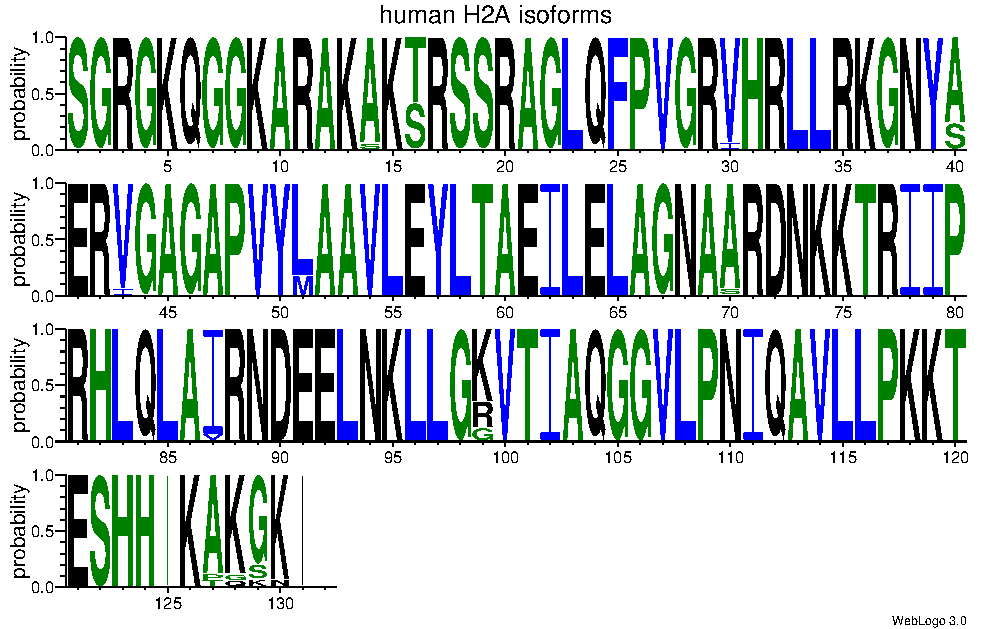
\includegraphics[width=\textwidth]{H2A_weblogo.png}
  \caption{WebLogo of all H2A sequences. The bottom line are the amino acids of H2AFJ whose sequence is different from any of the H2A proteins}
  \label{fig:h2a-weblogo}
\end{figure}


      \missingfigure{consensus and list of changes for each variant --- Marluzz paper style}

      \rewrite{comment on H2AFJ}

    \subsection{H2B}
      \begin{figure}
  \centering
  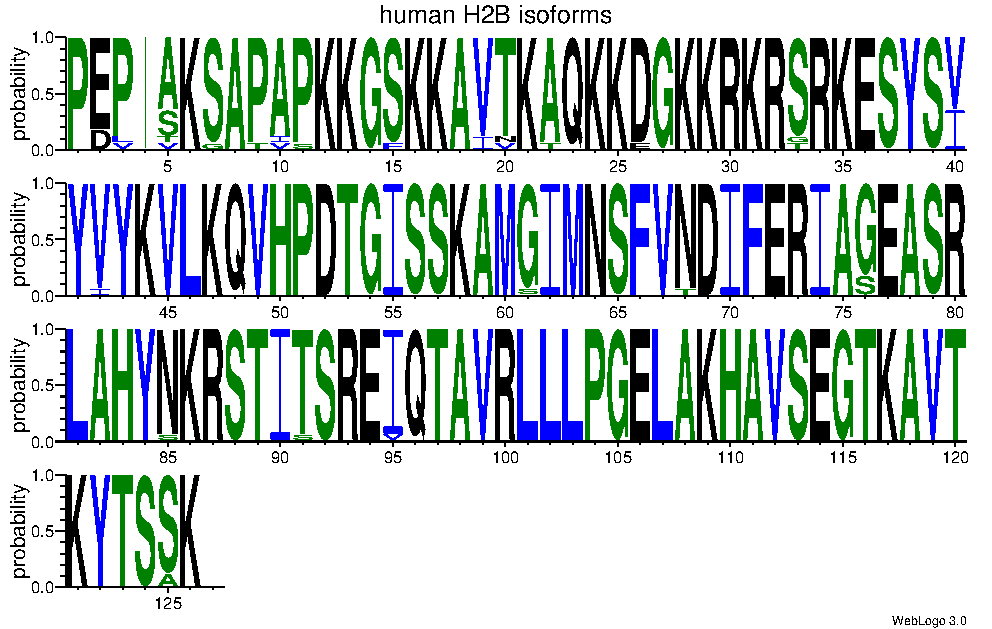
\includegraphics[width=\textwidth]{H2B_weblogo.png}
  \caption{WebLogo of all H2B sequences.}
  \label{fig:h2b-weblogo}
\end{figure}


      \missingfigure{consensus and list of changes for each variant --- Marluzz paper style}


    \subsection{H3}
      \begin{figure}
  \centering
  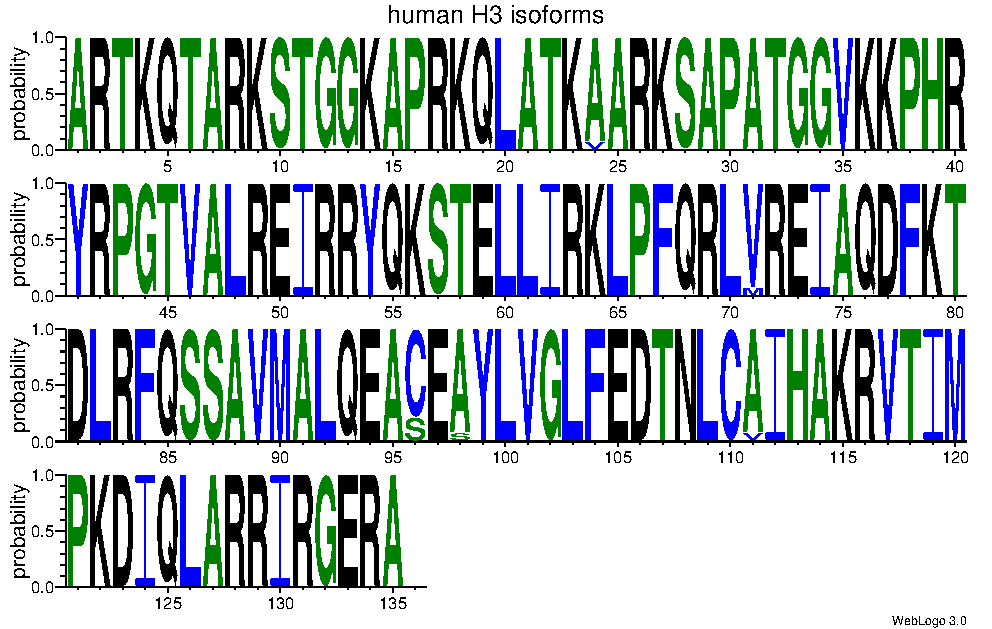
\includegraphics[width=\textwidth]{H3_weblogo.png}
  \caption{WebLogo of all H3 sequences.}
  \label{fig:h3-weblogo}
\end{figure}


      \missingfigure{consensus and list of changes for each variant --- Marluzz paper style}


    \subsection{H4}
      %% these should all be the same bu they are not. And there's an H4 in HIST4
      %% which is also present in mouse, which means has been conserved  in evolution
      With the exception of HIST1H4G, all H4 genes seem to encode the same protein. Even HIST4H4 which is the
      only gene on that ``cluster''.
      \begin{figure}
  \centering
  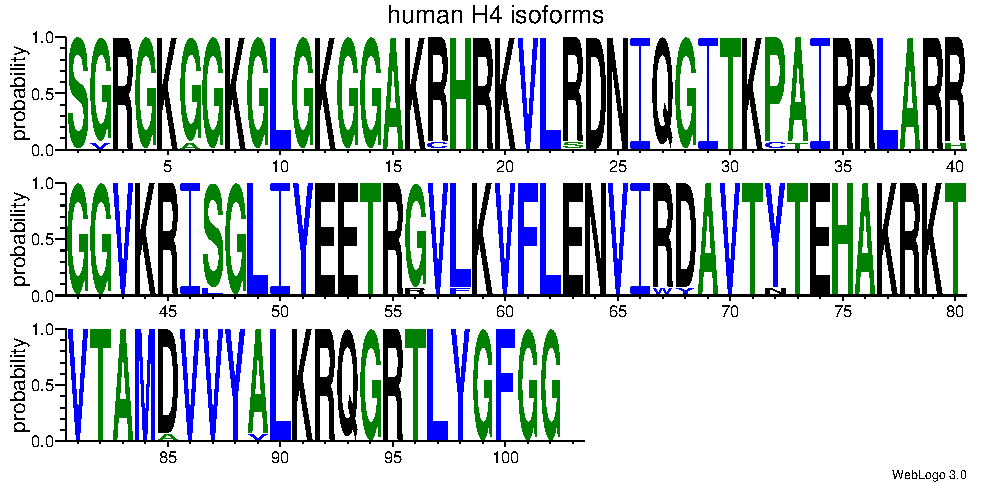
\includegraphics[width=\textwidth]{H4_weblogo.png}
  \caption{WebLogo of all H4 sequences. The non-conserved amino acids are all from one single gene --- HIST1H4G}
  \label{fig:h4-weblogo}
\end{figure}


      \begin{table}
  \centering
  \begin{tabular}{l | l}
    \multicolumn{2}{l}{Human histone H4 consensus (HIST1H4A/B/C/D/E/F/H/I/J/K/L, HIST2H4A/B, HIST4H4)} \\
    \hline
    \multicolumn{2}{l}{svrgkagkg lgkggakchr kvlsdniqgi tkctirrlar hggvkrilgl iyeetrrvfk vflenviwya vtntehakrk tvtamavvyv lkrqgrtl} \\
    \hline
    HIST1H4G   & G2V, G6A, R17C, R23S, P32C, A33T, R40H, S47L, G56R, L58F, R67W, D68Y, Y72N, D85A, A89V \\
  \end{tabular}
  \caption{Count of expected functional histone genes and proteins}
  \label{tab:H4-consensus}
\end{table}


%  \section{SNP's}
%    \rewrite{writing is dependent on what is found}


  \section{Characteristics of clusters}
    %% Talk about gene density of clusters, GC content, patterns of divergent promoters?
    %% HIST1 spans HIST1H2AA-HIST1H2BO 25726291-27861669; HIST2 spans HIST2H2BF-HIST2H2AB 149754245-149859466 (ensembl genome browser)
    HIST1 encodes 49 genes and 9 pseudogenes over a span of 2.3 megabasepairs and is the second
    most gene dense region on the megabase scale the genome (Xie 2003). It is located at the distal
    end of the major histocompatibility complex (MHC) in the extended class I region at chromosome
    6p21-22 (MHC consortium Nature 1999).

    HIST2 encodes 11 genes and 7 pseudogenes over a span of 105 kilobasepairs.

  \section{Proximity of stability and variation}
    %% Talk about how hyperrecombinational MHC next to HIST1, and deletion-duplication prone 1q21.1 adjacent to HIST2 (Brunetti-Pierri 2008)

  \section{Sequence extractor}
    To obtain the sequences for the alignment, curation, and IDs for the tables, a perl program using the
    BioPerl modules was written. This program performs a search on a specific database (Ensembl or GenBank), retrieves
    their sequences from the reference assembly, mRNAs and proteins. The sequences are saved in separate files whose
    names are either the gene/transcript/protein name or id.
    
    The program (sequence\_extractor) was submitted to the BioPerl project to be distributed together with it under the Perl artistic license

  \section{Reproducible research}
    While writing this document, we attempted to follow the principles of reproducible research \cite{reproducible-research-bioinformatics, reproducible-research-law}.
    We are also aware of the continuous development of databases and genetic knowledge. As such,
    the source code to replicate the tables and figures shown in this document are freely accessible
    online at gitorious. We hope that in the future, it can be used to create up to date information
    that reflects the current knowledge on the human histone genes.

\end{document}
